%% Run LaTeX on this file several times to get Table of Contents,
%% cross-references, and citations.

%% If you have font problems, you may edit the w-bookps.sty file
%% to customize the font names to match those on your system.

%% w-bksamp.tex. Current Version: Feb 16, 2012
%%%%%%%%%%%%%%%%%%%%%%%%%%%%%%%%%%%%%%%%%%%%%%%%%%%%%%%%%%%%%%%%
%
%  Sample file for
%  Wiley Book Style, Design No.: SD 001B, 7x10
%  Wiley Book Style, Design No.: SD 004B, 6x9
%
%
%  Prepared by Amy Hendrickson, TeXnology Inc.
%  http://www.texnology.com
%%%%%%%%%%%%%%%%%%%%%%%%%%%%%%%%%%%%%%%%%%%%%%%%%%%%%%%%%%%%%%%%

%%%%%%%%%%%%%
% 7x10
%\documentclass{wileySev}

% 6x9
\documentclass{wileySix}

\usepackage{graphicx}
\usepackage{listings}

\usepackage{color}
 
\definecolor{codegreen}{rgb}{0,0.6,0}
\definecolor{codegray}{rgb}{0.5,0.5,0.5}
\definecolor{codepurple}{rgb}{0.58,0,0.82}
\definecolor{backcolour}{rgb}{0.95,0.95,0.92}
 
\lstdefinestyle{mystyle}{
    backgroundcolor=\color{backcolour},   
    commentstyle=\color{codegreen},
    keywordstyle=\color{magenta},
    numberstyle=\tiny\color{codegray},
    stringstyle=\color{codepurple},
    basicstyle=\footnotesize,
    breakatwhitespace=false,         
    breaklines=true,                 
    captionpos=b,                    
    keepspaces=true,                 
    numbers=left,                    
    numbersep=5pt,                  
    showspaces=false,                
    showstringspaces=false,
    showtabs=false,                  
    tabsize=2,
    language=sh
}
 
\lstset{style=mystyle}

%%%%%%%
%% for times math: However, this package disables bold math (!)
%% \mathbf{x} will still work, but you will not have bold math
%% in section heads or chapter titles. If you don't use math
%% in those environments, mathptmx might be a good choice.

% \usepackage{mathptmx}

% For PostScript text
\usepackage{w-bookps}

%%%%%%%%%%%%%%%%%%%%%%%%%%%%%%%%%%%%%%%%%%%%%%%%%%%%%%%%%%%%%%%%
%% Other packages you might want to use:

% for chapter bibliography made with BibTeX
% \usepackage{chapterbib}

% for multiple indices
% \usepackage{multind}

% for answers to problems
% \usepackage{answers}

%%%%%%%%%%%%%%%%%%%%%%%%%%%%%%
%% Change options here if you want:
%%
%% How many levels of section head would you like numbered?
%% 0= no section numbers, 1= section, 2= subsection, 3= subsubsection
%%==>>
\setcounter{secnumdepth}{3}

%% How many levels of section head would you like to appear in the
%% Table of Contents?
%% 0= chapter titles, 1= section titles, 2= subsection titles, 
%% 3= subsubsection titles.
%%==>>
\setcounter{tocdepth}{2}

%% Cropmarks? good for final page makeup
%% \docropmarks

%%%%%%%%%%%%%%%%%%%%%%%%%%%%%%
%
% DRAFT
%
% Uncomment to get double spacing between lines, current date and time
% printed at bottom of page.
% \draft
% (If you want to keep tables from becoming double spaced also uncomment
% this):
% \renewcommand{\arraystretch}{0.6}
%%%%%%%%%%%%%%%%%%%%%%%%%%%%%%

%%%%%%% Demo of section head containing sample macro:
%% To get a macro to expand correctly in a section head, with upper and
%% lower case math, put the definition and set the box 
%% before \begin{document}, so that when it appears in the 
%% table of contents it will also work:

\newcommand{\VT}[1]{\ensuremath{{V_{T#1}}}}

%% use a box to expand the macro before we put it into the section head:

\newbox\sectsavebox
\setbox\sectsavebox=\hbox{\boldmath\VT{xyz}}

%%%%%%%%%%%%%%%%% End Demo


\begin{document}


\booktitle{}
\subtitle{D}

\authors{Difa Al Fansha\\
\affil{D4 TI 2C}
%Floyd J. Fowler, Jr.\\
%\affil{University of New Mexico}
}

%% Can use \\ if title, and edition are too wide, ie,
%% \offprintinfo{Survey Methodology,\\ Second Edition}{Robert M. Groves}

%%%%%%%%%%%%%%%%%%%%%%%%%%%%%%
%% 


\begin{introduction}

%% optional, but if you want to list author:

\introauthor{Rolly Maulana Awangga, S.T., M.T.}
{Informatics Research Center\\
Bandung, Jawa Barat, Indonesia}

Pada era disruptif  \index{disruptif}\index{disruptif!modern} 
saat ini. git merupakan sebuah kebutuhan dalam sebuah organisasi pengembangan perangkat lunak.
Buku ini diharapkan bisa menjadi penghantar para programmer, analis, IT Operation dan Project Manajer.
Dalam melakukan implementasi git pada diri dan organisasinya.

Rumusnya cuman sebagai contoh aja biar keren\cite{awangga2018sampeu}.

\begin{equation}
ABC {\cal DEF} \alpha\beta\Gamma\Delta\sum^{abc}_{def}
\end{equation}

\end{introduction}


\chapter{Sejarah Phyton}
{Pyhton merupakan bahasa open source yang memiliki aturan sintaksis tersendiri. Bahasa Pemrograman Python diciptakan oleh Guido Van Rossum berasal dari Belanda. Python mulai dikembangkan pada tahun 1990 di Stichting Mathematisch Centrum, Amsterdam -  Belanda sebagai kelanjutan dari bahasa pemrograman ABC.
Publikasi pertama Python dilakukan pada tahun 1991 dengan versi 0.9.0, tiga tahun kemudian (1994) lahir versi Pyton 1.0. Di tahun 1995, Guido pindah dari CWI ke Corporation For National Research Initiatives (CNRI) di Virginia Amerika sembari terus melanjutkan pengembangan Python.
Pada tahun 1995 - 2000 CNRI telah merilis Python versi 1.2, versi 1.3, versi 1.4, versi 1.5 dan versi terakhir 1.6. Pada Masa tersbut versi yang paling populer adalah versi 1.5.2.
Tahun 2000, Guido dan team pengembang pindah dengan membawa python ke Beopen.com. Beopen.com merupakan sebuah perusahaan komersil yang berasal dari California.Didalam naungan Beopen.com Guido dan tim membentuk PythonLabs, yang kemudian berhasil menciptakan Python 2.0. Setelah merilis Python 2.0, Guido dan team direkrut oleh Digital Creation (saat ini namanya Zope Corporation), sebuah perusahaan yang bergerak dibidang pembentukan produk open source untuk Content Managament System (CMS).
Di Tahun 2001, Guido dan team memutuskan melepaskan diri dari dari Digital Creation dan membentuk komunitas baru dengan nama Python Software Foundation (PSF). PSF adalah sebuah organisasi non-profit yang dibentuk sebagi pemegang hak cipta intelektual Python dan dengan begitu mencegah Python dimiliki oleh perusahaan komersial.
}


\chapter{Perbedaan phyton 2 dan 3}
Penulisan syntax(source code) yang berbeda, Python 2 dilengkapi dengan berbagai fitur programatikal seperti cycle-detecting garbage collector untuk mengotomasi manajemen memori, peningkatan dukungan untuk Unicode, list comprehension untuk membuat sebuah list berdasarkan list yang sudah ada. Unifikasi pada tipe data Python dan class ke satu hirarki terjadi pada rilis Python 2.2
Python 3 mengalami hambatan pada pengadopsiannya. Itu akibat dari tidak adanya backwards compatibility dengan Python 2. Hal ini membuat pengguna Python sangat berat hati untuk pindah ke versi 3 ini. Tambahannya, banyak sekali library yang hanya tersedia untuk Python 2., tapi setelah tim pengembangan di balik Python 3 telah berulang kali menjelaskan bahwa dukungan terhadap Python 2 akan segera dihentikan, dan semakin banyak libary disalin ke Python 3, maka penerapan Python 3 semakin lama semakin meningkat.

 	\chapter{Instalasi Phyton}
{
1. Setelah download selesai, kita akan mendapatkan file python-3.4.2.msi. File python-3.4.2.msi adalah file instalator python. File ini akan melakukan instalasi ke sistem windows.
}
\begin{figure}[!htbp]
\centering
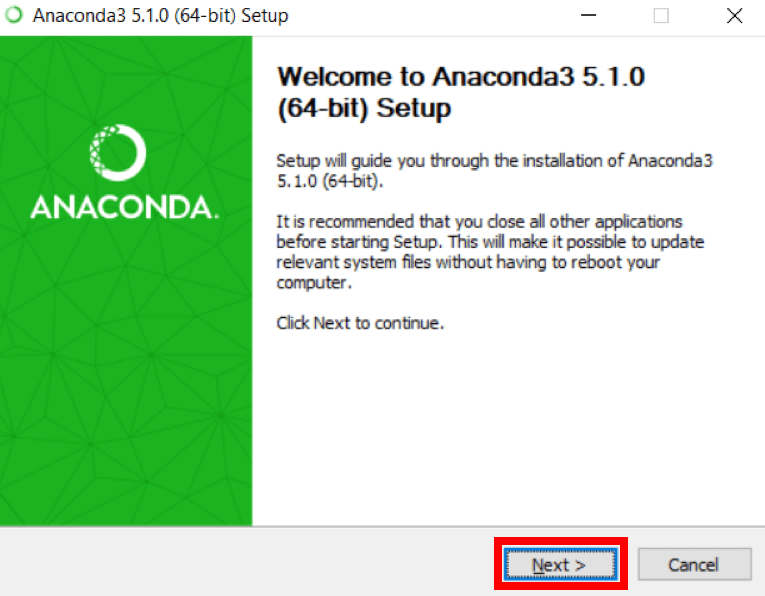
\includegraphics[width=3cm,height=3cm]{1.png}
\label{penanda}
\end{figure}

2. Pada tahapan ini kita akan diminta untuk memilih siapa saja yang boleh memakai python.
Pilih saja ‘Install for all users’ agar bisa dipakai untuk semua user di komputernya.
\begin{figure}[!htbp]
\centering
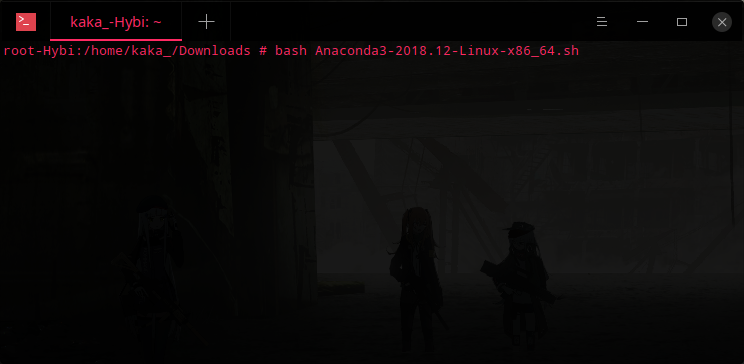
\includegraphics[width=3cm,height=3cm]{2.png}
\label{penanda}
\end{figure}

3.Tentukan lokasi python akan diinstal, kemudian klik next.
\begin{figure}[!htbp]
\centering
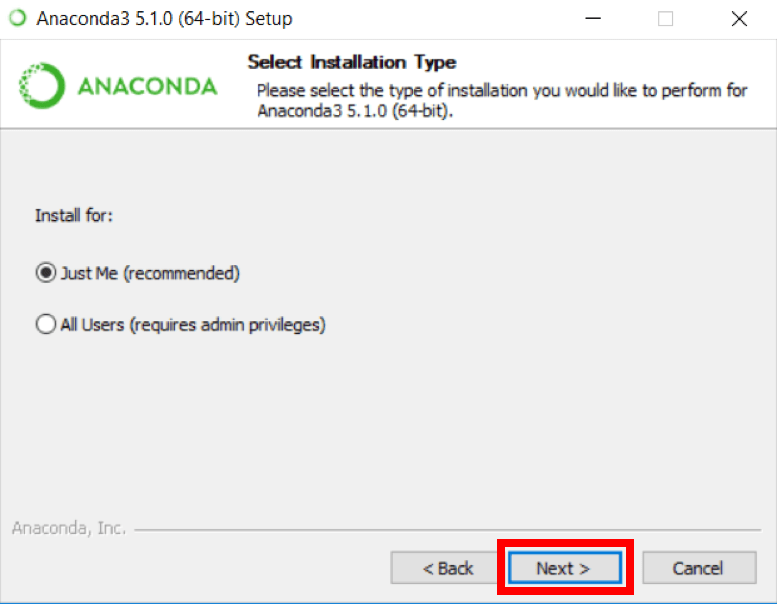
\includegraphics[width=3cm,height=3cm]{3.png}
\label{penanda}
\end{figure}

4.Pada tahapan ini, kita akan menentukan fitur-fitur yang akan diinstal.
Jangan lupa untuk mengaktifkan ‘Add python.exe to path’ agar perintah python dikenali pada CMD (Command Prompt).
\begin{figure}[!htbp]
\centering
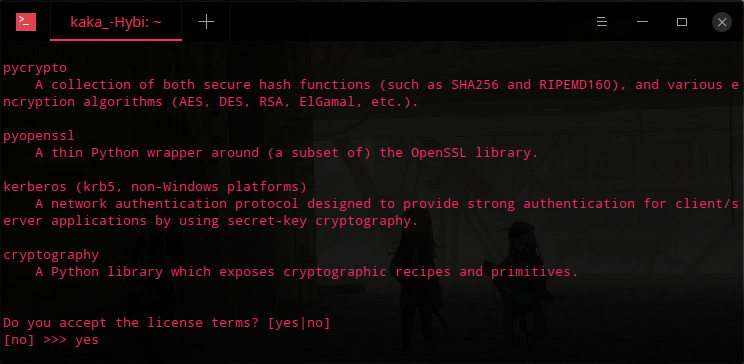
\includegraphics[width=3cm,height=3cm]{4.png}
\label{penanda}
\end{figure}

5.Selesai…
\begin{figure}[!htbp]
\centering
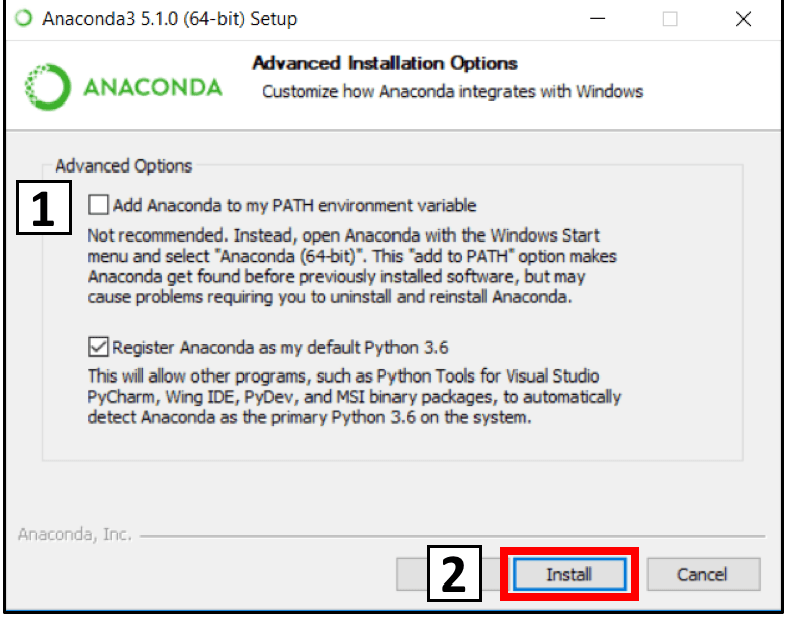
\includegraphics[width=3cm,height=3cm]{5.png}
\label{penanda}
\end{figure}



\bibliographystyle{IEEEtran} 
%\def\bibfont{\normalsize}


%%%%%%%%%%%%%%%
%%  The default LaTeX Index
%%  Don't need to add any commands before \begin{document}
\printindex

%%%% Making an index
%% 
%% 1. Make index entries, don't leave any spaces so that they
%% will be sorted correctly.
%% 
%% \index{term}
%% \index{term!subterm}
%% \index{term!subterm!subsubterm}
%% 
%% 2. Run LaTeX several times to produce <filename>.idx
%% 
%% 3. On command line, type  makeindx <filename> which
%% will produce <filename>.ind 
%% 
%% 4. Type \printindex to make the index appear in your book.
%% 
%% 5. If you would like to edit <filename>.ind 
%% you may do so. See docs.pdf for more information.
%% 
%%%%%%%%%%%%%%%%%%%%%%%%%%%%%%

%%%%%%%%%%%%%% Making Multiple Indices %%%%%%%%%%%%%%%%
%% 1. 
%% \usepackage{multind}
%% \makeindex{book}
%% \makeindex{authors}
%% \begin{document}
%% 
%% 2.
%% % add index terms to your book, ie,
%% \index{book}{A term to go to the topic index}
%% \index{authors}{Put this author in the author index}
%% 
%% \index{book}{Cows}
%% \index{book}{Cows!Jersey}
%% \index{book}{Cows!Jersey!Brown}
%% 
%% \index{author}{Douglas Adams}
%% \index{author}{Boethius}
%% \index{author}{Mark Twain}
%% 
%% 3. On command line type 
%% makeindex topic 
%% makeindex authors
%% 
%% 4.
%% this is a Wiley command to make the indices print:
%% \multiprintindex{book}{Topic index}
%% \multiprintindex{authors}{Author index}

\end{document}

